\documentclass[10pt,a4paper]{article}
\usepackage[margin=0.6in]{geometry}
\usepackage{amsmath,amssymb,amsfonts,stmaryrd}
\usepackage{xcolor}
\usepackage{enumitem}
\usepackage{tcolorbox}
\usepackage{multicol}
\usepackage{tikz}
\usetikzlibrary{trees, arrows.meta, positioning}
\usepackage{listings}
\usepackage{hyperref}

\definecolor{isabelleblue}{RGB}{0, 70, 140}
\definecolor{isabellekw}{RGB}{120, 0, 120}
\definecolor{boxbg}{RGB}{248, 249, 250}

\tcbset{
  colback=boxbg,
  colframe=isabelleblue,
  fonttitle=\bfseries\large,
  boxrule=0.8pt,
  arc=3pt,
  left=8pt,
  right=8pt,
  top=6pt,
  bottom=6pt
}

\title{\textbf{\huge Primitive Recursion on Algebraic Datatypes}\\[0.3em]
\large Lecture Notes}
\author{\textbf{Course:} Computer-Assisted Theorem Proving (7CCSACTP)}
\date{}

\begin{document}

\maketitle
\vspace{-1.5em}

\begin{tcolorbox}[title={1. Context \& Binary Tree Datatype Definition}]
\begin{multicols}{2}
\textbf{Previously Covered:}
\begin{itemize}[leftmargin=1.2em, itemsep=2pt]
    \item Isabelle interface \& basic reasoning (FW, BW, \texttt{subst}, induction on nats)
    \item Lists (recursive functions, structural induction)
    \item Algebraic datatypes (\texttt{nat}, \texttt{list}, \texttt{tree})
\end{itemize}

\textbf{This Video:}
\begin{itemize}[leftmargin=1.2em, itemsep=2pt]
    \item Primitive recursion on user-defined algebraic datatypes
\end{itemize}

\columnbreak

\textbf{Datatype Definition in Isabelle:}
\begin{center}
\texttt{datatype 'a tree = Leaf | Node "'a tree" 'a "'a tree"}
\end{center}

\textbf{Example Binary Search Tree (BST):}
\begin{center}
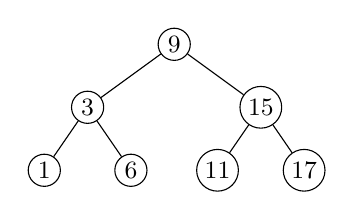
\begin{tikzpicture}[level distance=0.8cm, level 1/.style={sibling distance=2.2cm}, level 2/.style={sibling distance=1.1cm}, nodes={circle, draw, inner sep=1.5pt, font=\small}]
  \node {9}
    child { node {3}
      child { node {1} }
      child { node {6} }
    }
    child { node {15}
      child { node {11} }
      child { node {17} }
    };
\end{tikzpicture}
\end{center}
\end{multicols}
\end{tcolorbox}

\vspace{0.3em}

\begin{tcolorbox}[title={2. Primitive Recursive Functions: \texttt{tree\_set}}]
\textbf{Set of Elements in a Tree:}
\begin{align*}
\texttt{tree\_set Leaf} &= \emptyset \\
\texttt{tree\_set (Node l a r)} &= \text{insert } a \; (\texttt{tree\_set } l \cup \texttt{tree\_set } r)
\end{align*}

\textbf{Evaluation Trace on Example Tree:}
\begin{align*}
\texttt{tree\_set } T &= \text{insert } 9 \; (\texttt{tree\_set } T_3 \cup \texttt{tree\_set } T_{15}) \\
&= \text{insert } 9 \; (\text{insert } 3 \; (\texttt{tree\_set } T_1 \cup \texttt{tree\_set } T_6) \cup \text{insert } 15 \; (\texttt{tree\_set } T_{11} \cup \texttt{tree\_set } T_{17})) \\
&= \{1, 3, 6, 9, 11, 15, 17\}
\end{align*}
\end{tcolorbox}

\vspace{0.3em}

\begin{tcolorbox}[title={3. Inorder Traversal of Trees}]
\textbf{Definition of Inorder Traversal:}
\begin{align*}
\texttt{inorder Leaf} &= [] \\
\texttt{inorder (Node l a r)} &= (\texttt{inorder } l) \mathbin{@} [a] \mathbin{@} (\texttt{inorder } r)
\end{align*}

\textbf{BST Property:} If the tree is a Binary Search Tree (where for every node, all left subtree elements are $<$ node and all right subtree elements are $>$ node), then \texttt{inorder} yields a \textbf{sorted list}:
\[ [1, 3, 6, 9, 11, 15, 17] \]

\textbf{Step-by-step Evaluation Trace:}
\begin{align*}
\texttt{inorder } T_9 &= (\texttt{inorder } T_3) \mathbin{@} [9] \mathbin{@} (\texttt{inorder } T_{15}) \\
&= \big((\texttt{inorder } T_1) \mathbin{@} [3] \mathbin{@} (\texttt{inorder } T_6)\big) \mathbin{@} [9] \mathbin{@} (\texttt{inorder } T_{15}) \\
&= \big(([] \mathbin{@} [1] \mathbin{@} []) \mathbin{@} [3] \mathbin{@} ([] \mathbin{@} [6] \mathbin{@} [])\big) \mathbin{@} [9] \mathbin{@} \dots \\
&= ([1] \mathbin{@} [3] \mathbin{@} [6]) \mathbin{@} [9] \mathbin{@} ([11] \mathbin{@} [15] \mathbin{@} [17]) \\
&= [1, 3, 6, 9, 11, 15, 17] \quad \checkmark
\end{align*}
\end{tcolorbox}

\end{document}
